\documentclass[a4paper,11pt]{article}

\usepackage[utf8]{inputenc}

\usepackage{graphicx}
\usepackage{caption}
\usepackage{subcaption}

\usepackage{pgfplots}
\usepackage{float}
\usepackage{hyperref}
\usepackage{soul}
\hypersetup{
  colorlinks=true, % Enable colored links
  linkcolor=black, % Color for internal links
  urlcolor=black,  % Color for external links
  citecolor=black, % Color for citation links
  pdfborder={0 0 0}, % Remove border around links
}
\newcommand{\underlinehref}[2]{%
  \href{#1}{\ul{#2}}%
}
\pgfplotsset{compat=1.18}


\usepackage{minted}

\begin{document}

\title{
    \textbf{Arrays in C}
}
\author{Péter Herczku}
\date{Fall 2024}

\maketitle

\section*{Introduction}

The task is to analyze the performance and the time it takes to run array operations in C, such as randomly accessing an item, searching for an item and searching for duplicates.

\section*{Random access}

It is crucial to know how to measure execution time accurately.
We can use the built in clock in our computer for this purpose.
In C, we can get the current clock time using the {\tt clock\_gettime} function.
In the description of the assignment we were provided with the method {\tt nano\_seconds} that returns the elapsed time between two states in nanoseconds.
We will use this function to evaluate execution time.

First we can measure the time it takes to run a single element access.
After a few benchmarks, we can see that it varies between 0 and 300 nanoseconds.
The reason this is a relatively large number is that we are actually measuring the time it takes to call {\tt clock\_gettime} rather than the array access itself.
We can prove this assumption by only calling the {\tt clock\_gettime} function twice.
After looking at the benchmarks, we get the same result: the execution time is 0--300 ns.

Instead, we could perform the operation $n$ times, measure the time it takes to do that, and then divide this value by $n$.
Additionally, for the access to be random, we need to set up another array with random indexes.
We should do it before benchmarking the loop, otherwise we would measure the time it takes to generated a random number as well.

\begin{minted}{c}
// ... initialize variables, fill up arrays
clock_gettime(CLOCK_MONOTONIC, &t_start);
for (int i = 0; i < loop; i++) sum += array[idx[i]];
clock_gettime(CLOCK_MONOTONIC, &t_stop);
\end{minted}
\begin{table}[H]
  \begin{center}
    \begin{tabular}{l|c|c}
      \textbf{attempt} & \textbf{runtime}\\
      \hline
      1      &  2.0\\
      2      &  2.1\\
      3      &  2.0\\
      4      &  2.4\\
      5      &  3.2\\
    \end{tabular}
    \caption{Results of the first benchmark, runtime in nanoseconds}
    \label{tab:table1}
  \end{center}
\end{table}

\subsection*{Maximum, average and minimum time}
We can see that the runtime varies significantly.
In order to get a better understanding of how long it actually takes to run this operation, we can run it multiple times and measure the minimum, average and maximum time on different sizes of an array.

\begin{figure}[h]
  \centering
  \begin{subfigure}[b]{.5\textwidth}
    \centering
    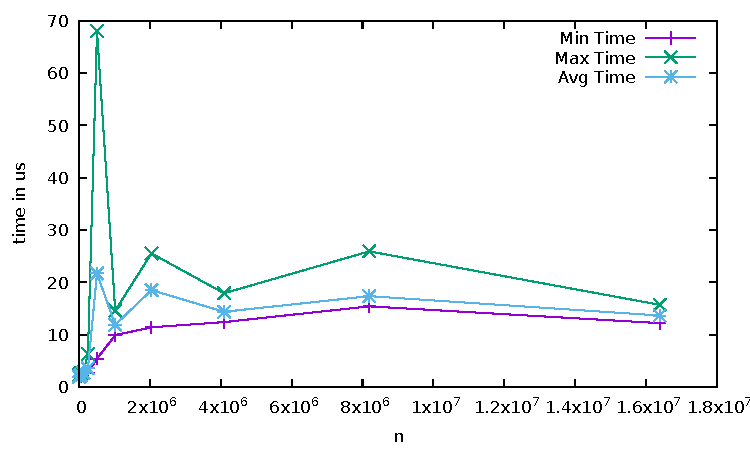
\includegraphics[width=\textwidth]{./min_max_average/data} % Adjust width or height as needed
  \end{subfigure}
  \caption{Graph of the minimum, maximum and average execution time on different sizes of arrays}
  \label{fig:graph_1}
\end{figure}

We observe a spike in the beginning, then the graph seems to consolidate but still continues to increase.
Let's take a closer look at the very beginning of the graph.

\begin{figure}[h]
  \centering
  \begin{subfigure}[b]{.5\textwidth}
    \centering
    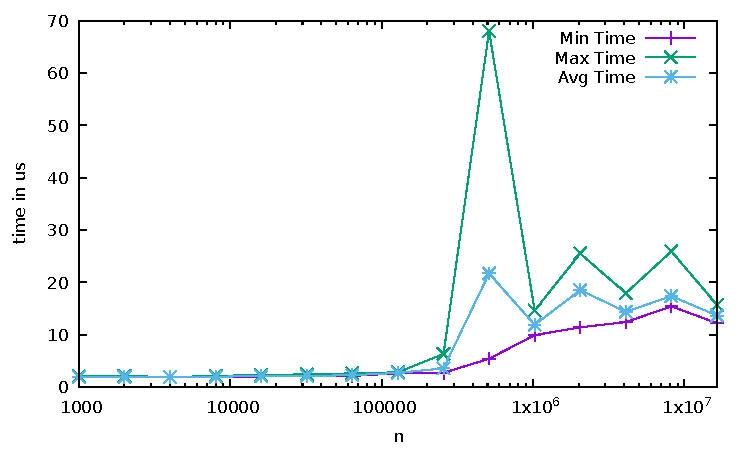
\includegraphics[width=\textwidth]{./min_max_average/data_2} % Adjust width or height as needed
  \end{subfigure}
  \caption{Graph of the minimum, maximum and average execution time on different sizes of arrays}
  \label{fig:graph_2}
\end{figure}

One can notice that the average execution time is highly affected by the maximum execution time.
However, the maximum execution time can be arbitrarily large, therefore we can neglect the maximum and average values.
The minimum time seems to be consistent in the beginning, but then starts increasing.
This might be an effect of several factors e.g cache misses.

\subsection*{Measuring median}

To find out more information, we can measure the median since it would give us a clearer picture.

\begin{figure}[h]
  \centering
  \begin{subfigure}[b]{.5\textwidth}
    \centering
    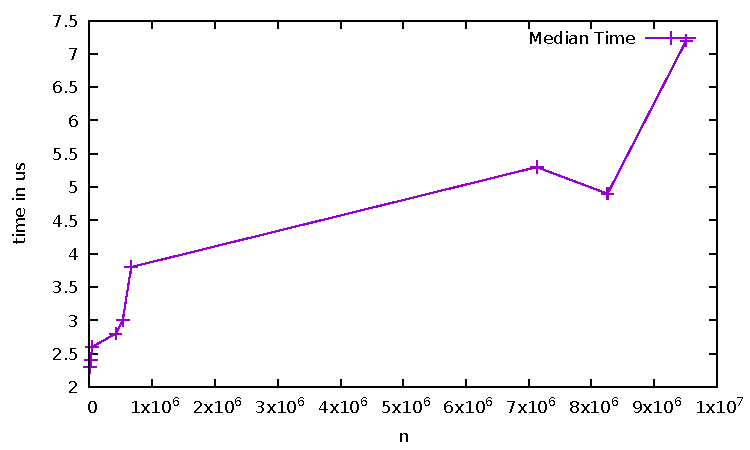
\includegraphics[width=\textwidth]{./median/data} % Adjust width or height as needed
  \end{subfigure}
  \caption{Graph of the median execution time on different sizes of arrays}
  \label{fig:graph_3}
\end{figure}

The conclusion of this graph is that the size of an array actually have an impact on the execution time of a random access in C.
If we are working with relatively small sizes of an array this difference is negligible, but cannot be on large sizes.

\section*{Search for an item}

In this task, we need to set up two arrays: one target array with random values and another one with keys that we want to search for.
When we set up the benchmark, we need to take into consideration that the arrays should not be sorted, and the size of the {\tt keys} array should be larger than the size of the target array.
Otherwise we might get false results because if the size of the keys is very small it may result in quickly finding the element we are looking for.
Let's run this benchmark with the provided method on different sizes of arrays, and analyze the results.

\begin{figure}[H]
  \centering
  \begin{subfigure}[b]{.5\textwidth}
    \centering
    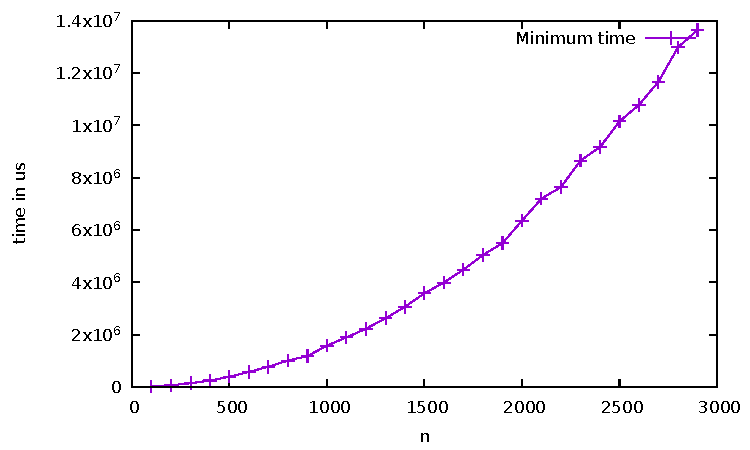
\includegraphics[width=\textwidth]{./search/data} % Adjust width or height as needed
  \end{subfigure}
  \caption{Graph of the minimum execution time for search}
  \label{fig:graph_4}
\end{figure}
The graph clearly shows that as we increase the number of elements in an array the execution time grows linearly as well.
In other words, the time complexity of this function is {\tt O(n)}.

\section*{Search for duplicates}

In this task, we have 2 arrays with the size {\tt n}, and we need to find all elements that are contained by both of the arrays.
With the given code from the assignment, we set up the benchmark accordingly.
In theory, we iterate through 2 arrays n times, so the complexity should be $O(n^2)$ .

\begin{figure}[H]
  \centering
  \begin{subfigure}[b]{.5\textwidth}
    \centering
    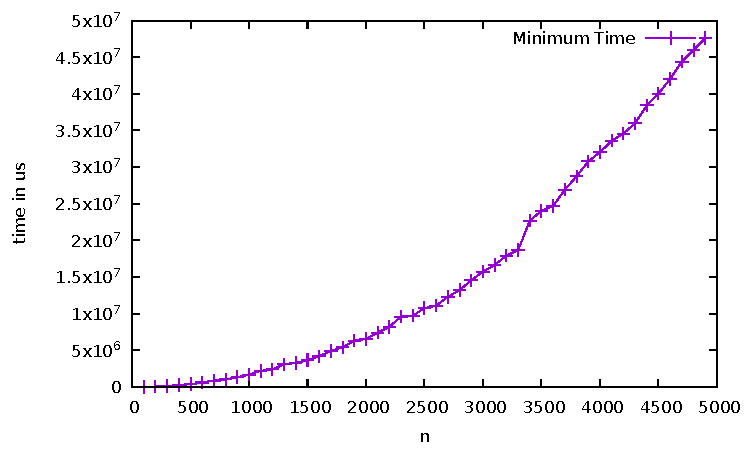
\includegraphics[width=\textwidth]{./duplicates/data} % Adjust width or height as needed
  \end{subfigure}
  \caption{Graph of the minimum execution time for duplicates}
  \label{fig:graph_5}
\end{figure}

Our graph indicates that our theoretical assumption was correct, and we got a quadratic relationship.
The time complexity of this function is truly $O(n^2)$.

\section*{GitHub}

I have uploaded the full project to \underlinehref{https://github.com/peterherczku/ID1021/tree/main/assignment-1}{my github repository}, where we can find the code I used to make this report.

\end{document}
